\documentclass[11pt]{article}

% Page layout
\usepackage[margin=1in]{geometry}

% Math
\usepackage{amsmath}
\usepackage{amssymb}

% Figures
\usepackage{graphicx}
\usepackage{subcaption}
\usepackage{float}

% Tables
\usepackage{booktabs}

% Links
\usepackage{hyperref}

% Better typography
\usepackage{microtype}

% Optional code listings
\usepackage{xcolor}
\usepackage{listings}

\definecolor{codebackground}{RGB}{245, 245, 245}
\definecolor{codeborder}{RGB}{210, 210, 210}
\definecolor{codecomment}{RGB}{80, 130, 80}
\definecolor{codekeyword}{RGB}{40, 80, 160}
\definecolor{codestring}{RGB}{160, 70, 70}

\lstdefinestyle{python}{
    language=Python,
    basicstyle=\ttfamily\small,
    backgroundcolor=\color{codebackground},
    frame=single,
    rulecolor=\color{codeborder},
    keywordstyle=\color{codekeyword},
    commentstyle=\color{codecomment},
    stringstyle=\color{codestring},
    showstringspaces=false,
    breaklines=true,
    columns=fullflexible,
    keepspaces=true,
    tabsize=4,
    xleftmargin=0.5em,
    xrightmargin=0.5em,
    framexleftmargin=0.5em,
    framexrightmargin=0.5em,
}

\lstset{
    basicstyle=\ttfamily\small,
    frame=single,
    breaklines=true,
    columns=fullflexible
}

\title{Learning Procedural World Generation}
\author{Tyler Forgione}
\date{\today}

\begin{document}

\maketitle
\tableofcontents

\section{Introduction}

This document records my progress while learning procedural world generation, including the algorithms, design decisions, experiments, and results developed throughout the project.

\section{Noise Generation}

A common way to generate a 2D map or terrain is to use noise. We often think of noise as a random signal. We think of static on a Television screen when the cable goes out. That is a very specific kind of noise, called white noise.

\subsection{White Noise}

In 2D, white noise is a grid in which each cell has a random intensity, generally between 0 and 1. The result is a mess of white and black dots on a map that means little. We can create white noise very easily by randomly sampling values in [0, 1] and assigning them to cells on a grid. Below is a Python implementation of white noise using NumPy:

\begin{lstlisting}[style=python]
def white_noise(height, width, seed):
    rng = np.random.default_rng(seed)
    return rng.random(size=(height, width), dtype=np.float32)
\end{lstlisting}

This results in an output like that in Figure \ref{fig:white-noise}. As is obvious, this is completely random! There is no meaning behind the colour of any dot. If we were to map this in 3D, we'd get mountains with essentially $90\deg$ angles with the ground below them. There would be no slope to any hill, mountain, or valley. To show this, I've plotted the exact same noise map in 3D. Figure \ref{fig:white-noise-3d} shows the terrain we'd get if only using white noise in our generation.

\begin{figure}[htbp]
    \centering

    \begin{subfigure}{0.48\textwidth}
        \centering
        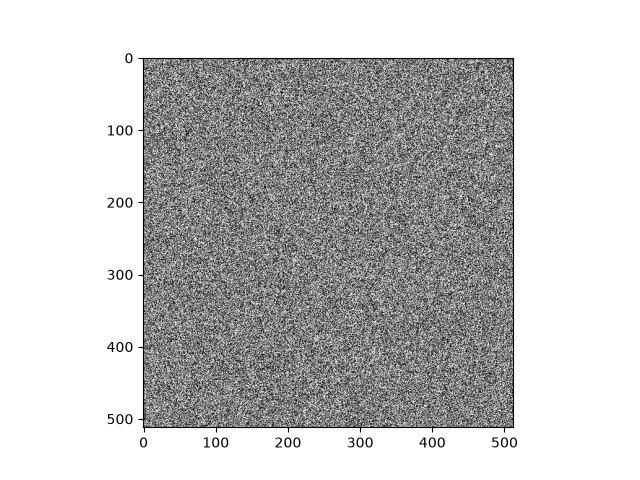
\includegraphics[width=\textwidth]{images/whitenoise.png}
        \caption{White noise}
        \label{fig:white-noise}
    \end{subfigure}
    \hfill
    \begin{subfigure}{0.48\textwidth}
        \centering
        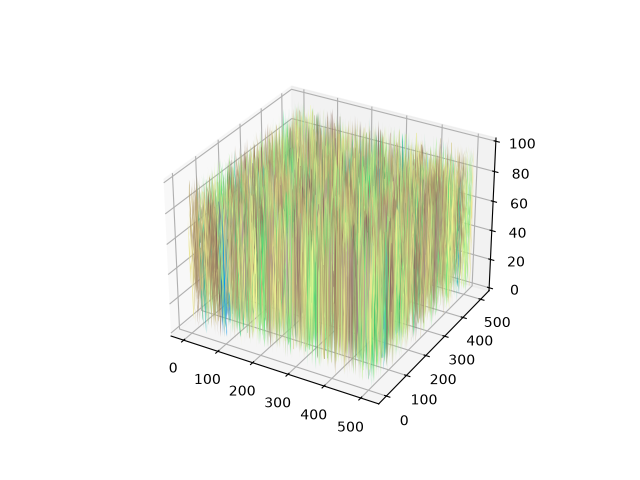
\includegraphics[width=\textwidth]{images/whitenoise_3d.png}
        \caption{White noise plotted in 3D}
        \label{fig:white-noise-3d}
    \end{subfigure}

    \caption{White noise in 2D and 3D}
    \label{fig:white-noise-comparison}
\end{figure}

Since terrain needs some sort of synchronicity between adjacent points, white noise won't cut it. Luckily, there are other noise algorithms that provide far better results.

\subsection{Value Noise}

The idea behind value noise is simple: create a grid of random values at integer points $(x, y)$ and interpolate between them to achieve smooth transitions. Essentially, for any integer point, we must find the surrounding lattice points (4 corners of the cell) and interpolate between them.

Just doing this, however, does not achieve the smoothest of transitions. Without using smoothing, we still may get clunky or jagged edges. Thus, the final piece of the puzzle for value noise is an additional smoothing on the weight parameter in linear interpolation.

Mathematically it's this: we begin with a smoothing function, the cubic Hermite smoothstep

\begin{equation}
    S(t)=3t^2 - 2t^3
    \label{eq:cubic-hermite}
\end{equation}

We can then define the following:

\begin{align*}
    s=S(u) &  &
    t=S(v)
\end{align*}

Next, we can use our linear interpolation function

\begin{equation}
    L(a,b,t)=a+t(b-a)
    \label{eq:lerp}
\end{equation}

to interpolate the top two points and bottom two points horizontally

\begin{align*}
    T=L(v_{00}, v_{10}, s) \\
    B=L(v_{01}, v_{11}, s)
\end{align*}

and to interpolate these two vertically

\[
    N(x, y) = L(T, B, t)
\]

Substituting and expanding gets us

\begin{equation}
    N(x, y) = L(L(v_{00}, v_{10}, S(u)), L(v_{01}, v_{11}, S(u)), S(v))
    \label{eq:value-noise}
\end{equation}

Where $S$ and $L$ are equation \ref{eq:cubic-hermite} and equation \ref{eq:lerp}, respectively.

One other factor we may want to take into account is the wavelength, which is the distance between adjacent lattice points. The lower the wavelength, the higher the spatial frequency of the noise. As wavelength goes to $1$, the closer we get to white noise because there will be less interpolation between lattice points.

From equation \ref{eq:value-noise}, we can replace $x$ and $y$ with $x' = \lfloor \frac{x}{\lambda} \rfloor$ and $y' = \lfloor \frac{y}{\lambda} \rfloor$, where $\lambda$ is the wavelength.

That just about wraps up value noise. The only other possible change is to use octaves and summing up noise from different octaves to create a more detailed terrain.

\subsection{Fractal Noise}

\section{Terrain Generation}

\subsection{Heightmaps}

\section{Experiments}

\section{Notes and Future Work}

\end{document}